\section{Crawler}
We implemented a crawler that visits other nodes and request the full chain of that node.
The crawler was built to be used for the experiments and
is a first step in a more sophisticated crawler that will help to solve the known vulnerabilities.
These vulnerabilities will be described in chapter \ref{problems}.

\subsection{Recursively request blocks}
Dispersy provides a list of other nodes that were recently found
and can report when the node itself is found by another node.
Both are sources of destinations nodes that the crawler will visit
and request the chain from.

The crawler will first request from a node the block with sequence number $-1$.
This denotes that he wants the latest block in his chain.
The node returns this block to the crawler.
The crawler will persist the block if it is not yet know.

The newly retrieved block is chained to two blocks with the previous hashes.
The crawler will check if these blocks are present in the database.
If any block is not present,
then the crawler will request that particulair block.
The peer, to whom the block belongs to, has to be known in Dispersy.
If the peer is not known, the block is ignored.
This is done recursively untill the crawler reaches the genesis block of the chain.
In this fashion a breadth first search is implemented for any unknown block
that is present in the chain before the latest block.

The crawl tries to aggregrate as much blocks as possible.
But it gives no certainty that the full MultiChain is collected.
The crawler is able to crawl a disconnected MultiChain,
if for every disconnected partition a peer is known by Dispersy.

\begin{figure}
	\centerline{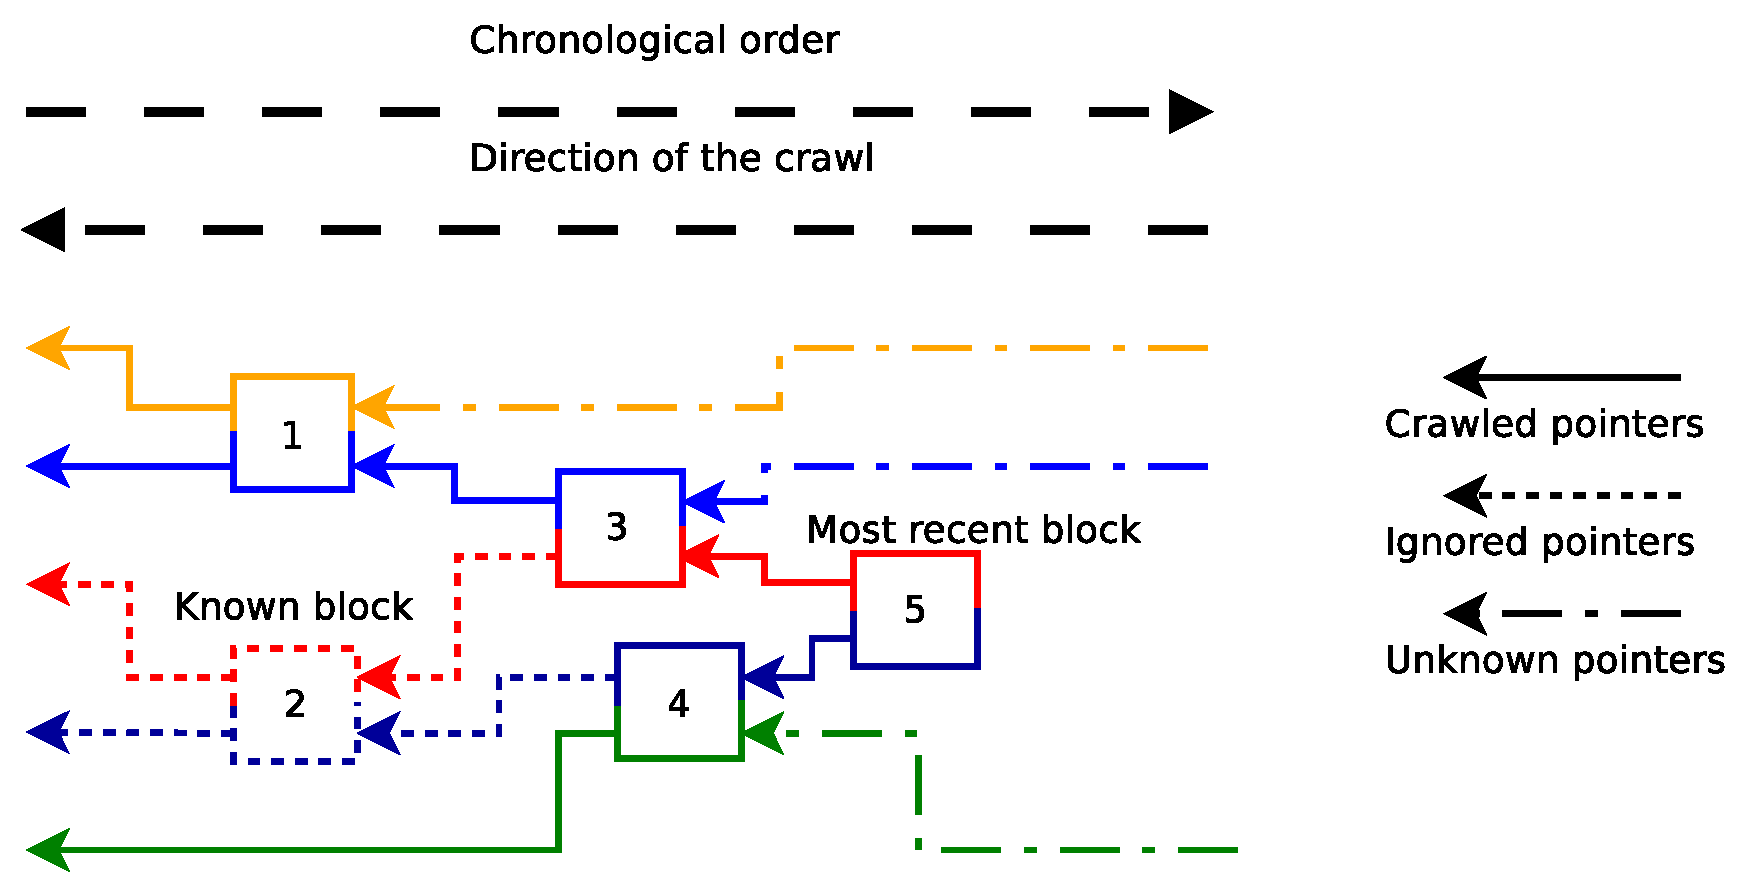
\includegraphics[scale=0.3]{design/figs/crawler-version2.eps}}
	\caption{Example of the crawler looking for unknown blocks. The crawler retrieves the most recent block and crawls older blocks.}
	\label{fig:crawler-example}
\end{figure}

An example can be seen in Figure \ref{fig:crawler-example}.
In this example the line arrows denote paths that the crawler follows,
dotted lines are paths that the crawler ignores,
half dotted lines are paths that the crawler will not know about.
Block 2 is already known by the crawler.
Block 5 is retrieved first by the crawler and the crawler sees hash links to block 3 and 4.
These are retrieved and the block finds links to block 1 and 2.
Because block 2 is already known, it is ignored.
Only block 1 is retrieved.
The crawler continues to follow the links further outside the displayed example.
The half dotted lines are not know by the crawler untill a block is retrieved that contains these paths.
The crawler will retrieve these blocks if for example the most recent block is requested.

\subsection{Recreation over retransmission}
An effort was made to try to reuse code of the community for the crawler and to not introduce another payload type in the community.
The attempt would reuse payload classes and authentication classes already used in the community for the creation of blocks.
This effort failed, because Dispersy cannot handle recreation of messages well
and would invalidate blocks that were recreated.

As said before, Dispersy also keeps tracks of messages received.
The messages containing a block requested by the crawler could be retrieved and retransmissioned forward
instead of being retrieved from the MultiChain database itself.
This would eliminate the need to construct a message and encode the message before it could be send,
because the encoded format is saved and can be retrieved and send immediately.
This was not used as it would be impossible to distinguish messages received as an response to a signature request or a crawler request.
The two types of responses cannot be processed in the same way.
A response to a signature requests has to influence the way a node responds to interactions
and a crawler response should not.

In the end, the crawler uses recreation of a block from the local database and uses a new payload type to forward blocks.
The main reasons this implementation was chosen is
that implemenation was very simple and had none of the above mentioned problems.
Maintainabillity is also much easier this way
as different types of messages are not using the same functions to be received in the code.
This might not be known by a new programmer working with the code.

\subsection{Improvements}
The crawler is a first, simple step towards a more sophisticated crawler.
Tribler has implemented already more sophisticated crawlers for Bartercast
and these techniques can be reused for the MultiChain crawler.
For example bloom filters can be used in conjunction with the knowledge
that every record is a part of the chain to quickly request multiple blocks\cite{broder-bloomfilter}\cite{logiotatidis-splash}.
Blocks could also be send in a more efficient way by sending multiple blocks per message.
Secondly, blocks that belong to a different node than the crawled node are requested,
but the location of this different node is only known by chance.
Dispersy only keeps track of 20 peers at any time, so the chance is low that the node is among these nodes.
The chance can be improved by asking if the first contacted node knows the location of the different node.


